\section{Funcionamiento del programa}
\subsection{Funcionamiento de Software}

El código se implementará en dos etapas, la primera consiste en una etapa de control y la segunda en una etapa de seguimiento, ambas son completamente independientes la una de la otra.

\begin{itemize}
    \item \textbf{Seguimiento}: La etapa de seguimiento implementa el sensor de línea, la idea es regular el funcionamiento de los motores de acuerdo a la corrección que ha de ser necesario para mantener el vehículo encima de la línea a seguir, y garantizar de esta forma seguimiento del trazo deseado. Toda la implementación de este código se hará programada en el IDE de Arduino puesto que al ser la etapa semi autónoma del proyecto no requiere de ningún comando desde un centro de control para la toma de decisiones. 
    Esta etapa de seguimiento implementa 3 sensores, uno para reconocer la línea a seguir, y dos sensores de obstáculo, uno de ellos encargado de detectar obstáculos frente al vehículo para su remoción, y el otro sensor para reconocer cuando se llega al final del recorrido.
    
    \item \textbf{Control}: La etapa de control se encarga de manejar el funcionamiento de los motores de manera remota mediante un módulo bluetooth, la idea es enviar datos desde un programa en C a través del puerto serial. Dependiendo de qué dato sea enviado, el vehículo llevará a cabo distintos movimientos. El programa en C cuenta con distintas funciones que permiten controlar el puerto serial, al cual se conecta el módulo bluetooth, son dos funciones en total. La primera se encarga de inicializar el puerto serial, una vez inicializado se puede utilizar la otra función, que se utiliza para escribir en el puerto serial, de esa forma se establece una comunicación unidireccional. Dichas funciones serán implementadas en una interfaz gráfica que simula un control remoto, la idea es controlar el vehículo con el teclado, y con la interfaz visualizar los movimientos que realiza el vehículo.
\end{itemize}

\subsubsection{Interfaz}
La interfaz utilizada en este proyecto utiliza una herramienta llamada GTK, más específicamente GTK+-2.0, la cual es una multiplataforma de herramientas que permite crear interfaces de gráficas de uso para el usuario. Este ofrece un set completo de widgets, estos siendo pequeñas aplicaciones con accesos directos permitiendo la sencilla visualización de las funciones principales utilizadas en determinado programa o documento. También es adaptable a proyectos que van desde pequeñas herramientas hasta aplicaciones muy completas permitiendo su funcionalidad. Se usa en diferentes sistemas operativos tales como Windows, GNU/Linux and Unix, OSX e inclusive dispositivos móviles. Escrito en lenguaje C, y permitido además en C++, Perl y Python. \cite{interfaz}
    \begin{itemize}
        \item\textbf{Función para crear las características del botón:}
        Esta es la función tipo Gtkwidget que recibe que la tabla o matriz interna se establecerá en la ventana de la interfaz que contendrá los botones, un dato char que es el tamaño de los botones, además dos datos de  tipo int que son la posición en fila y columna de los botones, luego esta hace un gtk button new with label que es el botón, además del color, de la posicion en la interfaz y  gtk widget show que hace que retorne todas esas características del botón.
        
\begin{lstlisting}

GtkWidget *CreateButton(GtkWidget *table, char *szLabel, int row, int column)
{
        GtkWidget *button;

        button = gtk_button_new_with_label(szLabel);

        gtk_signal_connect(GTK_OBJECT(button), "clicked",
                           GTK_SIGNAL_FUNC(button_clicked), szLabel);

        GdkColor color;

        gdk_color_parse("red", &color);

        gtk_widget_modify_bg(GTK_WIDGET(button), GTK_STATE_NORMAL, &color);

        gtk_table_attach(GTK_TABLE(table), button,
                         column, column + 1,
                         row, row + 1,
                         GTK_FILL | GTK_EXPAND,
                         GTK_FILL | GTK_EXPAND,
                         10, 15);

        gtk_widget_show(button);

        return (button);
}
\end{lstlisting}
        \item\textbf{Función que crea el botón en la interfaz:}
        Esta función es de tipo void que recibe la tabla o matriz interna, se establecerá en la ventana de la interfaz que contendrá los botones, luego se crea un dato que hace que el ciclo for recorra la lista de los botones y con ayuda de la función CreateButton se cree el botón y aparezca en la interfaz.
        
\begin{lstlisting}
void CreateControlButtons(GtkWidget *table)
{
        int nIndex;

        for (nIndex = 0; nIndex < numbuttons; nIndex++)
        {

                buttonList[nIndex].widget =
                    CreateButton(table,
                                 buttonList[nIndex].szLabel,
                                 buttonList[nIndex].row,
                                 buttonList[nIndex].col);
        }
}
\end{lstlisting}

 \item\textbf{Función para poder usar los botones del teclado:}
        Esta función es de tipo void que recibe un widget, un evento y la información del teclado, hace uso de un ciclo for que da busqueda entre los botones, y una condición if que permite si la pulsación de la tecla es el primer carácter de un botón y la longitud de la etiqueta del botón es de 1, entonces permite el retorno que conecta el botón presionado en el teclado con la interfaz gráfica y la tarea asociada.
    

\begin{lstlisting}
void key_press(GtkWidget *widget,
               GdkEventKey *event,
               gpointer data)
{
        int npressed;

        for (npressed = 0; npressed < numbuttons; npressed++)
        {
                if (event->keyval == buttonList[npressed].szLabel[0] &&
                    buttonList[npressed].szLabel[1] == (char)0)
                {
                        gtk_widget_grab_focus(buttonList[npressed].widget);
                        gtk_button_clicked(GTK_BUTTON(buttonList[npressed].widget));
                        return;
                }
        }
}

\end{lstlisting}

        \item\textbf{Función para clickear el botón y realizar una tarea:}
        Es la función de tipo void que recibe un widget y la información, este contiene dos datos tipo int los cuales son el baud rate y el puerto, dos punteros de tipo char, el str se encarga de agarrar el texto del botón y la información, además contiene la ventana que contiene la interfaz, luego varias condiciones if que permiten comparar el botón clickeado o presionado en el teclado que conecta con el puerto serial y retorna la tarea que realiza el vehículo. 
        
\begin{lstlisting}
void button_clicked(GtkWidget *widget, gpointer data)
{
        int baudrate = 115200;
        int port;
        port = serialport_init("/dev/rfcomm0", baudrate);

        char ch = *((char *)data);
        char *str;
        GtkWidget *window;
        window = gtk_window_new(GTK_WINDOW_TOPLEVEL);

        str = (char *)data;

        if (strcmp(str, "w") == 0)
        {

                char a = 'w';
                const char *ptr = &a;
                serialport_write(port, ptr);

                return;
        }
        else if (strcmp(str, "a") == 0)
        {

                char a = 'a';
                const char *ptr = &a;
                serialport_write(port, ptr);

                return;
        }
        else if (strcmp(str, "d") == 0)
        {

                char a = 'd';
                const char *ptr = &a;
                serialport_write(port, ptr);

                return;
        }
        else if (strcmp(str, "s") == 0)
        {

                char a = 's';
                const char *ptr = &a;
                serialport_write(port, ptr);

                return;
        }
        else if (strcmp(str, "1") == 0)
        {

                char a = '1';
                const char *ptr = &a;
                serialport_write(port, ptr);

                gtk_label_set(GTK_LABEL(label), "Control Mode");
                return;
        }
        else if (strcmp(str, "2") == 0)
        {

                char a = '2';
                const char *ptr = &a;
                serialport_write(port, ptr);

                gtk_label_set(GTK_LABEL(label), "Waiting mode");
                return;
        }
        else if (strcmp(str, "3") == 0)
        {

                char a = '3';
                const char *ptr = &a;
                serialport_write(port, ptr);

                gtk_label_set(GTK_LABEL(label), "Tracking mode");
                return;
        }
        else if (strcmp(str, "y") == 0)
        { //scalubur time

                char a = 'e';
                const char *ptr = &a;
                serialport_write(port, ptr);

                return;
        }
        else if (strcmp(str, "b") == 0)
        { //buzzer

                char a = 'b'; 
                const char *ptr = &a;
                serialport_write(port, ptr);

                return;
        }
        else if (strcmp(str, "t") == 0)
        { //trompo

                char a = 't';
                const char *ptr = &a;
                serialport_write(port, ptr);

                return;
        }

      
}
\end{lstlisting}

        \item\textbf{Función para cerrar la ventana y finalizar el programa:}
        Es una función de tipo int que recibe un widget y la información, que utiliza un gtk main quit que retorna el cierre de la ventana y, por ende, del programa.
        
\begin{lstlisting}
int CloseAppWindow(GtkWidget *widget, gpointer data)
{
        gtk_main_quit();

        return (FALSE);
}
\end{lstlisting}
        
    \end{itemize}   
   

\subsubsection{Comunicación}
La comunicación cuenta con varios elementos fundamentales.
\begin{itemize}
    \item\textbf{Módulo bluetooth HC-05:} El módulo bluetooth permite establecer una comunicación inalámbrica para poder manipular los movimientos del vehículo por medio de una interfaz en el computador. El módulo se configura utilizando los comandos AT, los cuales permiten establecer el modo de operación del módulo, el nombre, la contraseña, el baud rate, etc.
    \item\textbf{Blueman:} Es una aplicación que permite gestionar dispositivos bluetooth, de manera que se puedan enlazar a un computador y además permite conectarlos a un puerto serial para poder enviar datos desde algún programa.
    \item\textbf{Programa en C:} En un programa en C se implementaron dos funciones, una para poder inicializar el puerto serial y la otra para poder escribir en el puerto serial. Dichas funciones se explican con más detalle a continuación.
\end{itemize}                         
\begin{itemize}
    \item\textbf{Función para inicializar el puerto serial:}
    Esta función recibe de parámetros el nombre del puerto en el que está conectado el módulo bluetooth y el baud rate que éste utiliza. Luego, se implementa otra función que permita abrir el puerto para poder escribir y leer de él. En caso de que no se encuentre nada conectado al puerto, imprime un error y falla la inicialización. Si el puerto está conectado a algún dispositivo, entonces retorna la función que abre el puerto. La función que abre el puerto está implementada en las bibliotecas utilizadas.
    \begin{lstlisting}
    int serialport_init(const char *serialport, int baud)

{

        int fd;
        fd = open(serialport, O_RDWR | O_NOCTTY);
        if (fd == -1)
        {

                perror("init_serialport: Unable to open port ");

                return -1;
        }
        return fd;
}
    \end{lstlisting}
    \item\textbf{Función para escribir en el puerto serial:} Esta función recibe de parámetros la función anterior y el caracter que se desea escribir en el puerto serial. Luego, con el puerto ya inicializado y con el caracter que se desea enviar, entonces se escribe dicho caracter en el puerto. Ya en el arduino se implementan otras funciones que permitan leer estos datos, y el vehículo pueda realizar sus distintas acciones.
    \begin{lstlisting}
    int serialport_write(int fd, const char *str)

{
        int len = strlen(str);

        int n = write(fd, str, len);

        if (n != len)

                return -1;
        return n;
}
    \end{lstlisting}
\end{itemize}

\subsubsection{Vehículo}
En esta sección se presentan únicamente algunas de las funciones más importantes generadas en el código fuente \´´AuveTA.ino"  para el vehículo, además del loop de dicho código en arduino, esto debido a que el mismo tiene una extensión considerable y que se encuentra bien comentado y documentado en el \textit{Doxygen}. Podrá encontrar el código completo y comentado en la sección de anexos al final del trabajo, específicamente en el apartado \textit{\´´6.1.1. AuVeTA.ino"}, además de poder consultar el \textit{Doxygen} disponible en: \textit{https://gitlab.com/UCR-EIE/IE-0117/i-2019/g0/tree/master/AuVeTAº\%20Proyecto\%20Plataformas. }

\begin{itemize}

    \item \textbf{ Setup general:} En la programación de arduino tenemos dos componentes estructurales esenciales, una de ellas es el setup. Acá es donde se inicializan por ejemplo, las comunicaciones seriales, asigna funcionamiento de entrada o salida a los pines digitales y analógicos, se declaran objetos a utilizar como myServo de la biblioteca servo.h. Esta es una estructura por la que se pasa solamente una vez cuando se reinicie el arduino. 
    \begin{lstlisting}
void setup(){
  //Seteo para comunicación serial USB:
  Serial.begin(9600);

  ////Seteo para comunicación serial Bluetooth:
  mySerial.begin(115200);

  //Set for digital pins:
  pinMode(R, OUTPUT);
  pinMode(G, OUTPUT);
  pinMode(B, OUTPUT);
  pinMode(servo_pin, OUTPUT);
  pinMode(obstacle_pin, INPUT);
  pinMode(track1_pin, INPUT);
  pinMode(final_sensor, INPUT);
  pinMode(buzzer, OUTPUT);
  pinMode(motorL_forward, OUTPUT);
  pinMode(motorL_reverse, OUTPUT);
  pinMode(motorR_forward, OUTPUT);
  pinMode(motorR_reverse, OUTPUT);

  //Seteo para servo
  myServo.attach(servo_pin);
  myServo.write(servo_close);
  delay(500);
  myServo.detach();
  
  //Seteo inicial de motores en cero
  digitalWrite(motorR_forward, 0);
  digitalWrite(motorL_forward, 0);
  digitalWrite(motorR_reverse, 0);
  digitalWrite(motorL_reverse, 0);
}
\end{lstlisting}
    \item \textbf{ Loop general} Como ya se mencionó antes, en la programación de arduino tenemos dos componentes estructurales esenciales, uno de ellos es el loop. Acá es donde se ejecutan y convocan las funciones principales del código para el vehículo. Esta es una estructura, que a diferencia del setup, se repite una y otra vez hasta que se reinicie el arduino. 
    \begin{lstlisting}
void loop()
{   
//luz roja en "Waiting Mode":
  digitalWrite(R, LOW);
  digitalWrite(G, LOW);
  digitalWrite(B, LOW);
//Revisión de puerto serial disponible
  if (mySerial.available())
  {
//Lectura Serial para selección de modo: 3 -> "Trackig Mode" || 2 -> "Waiting Mode" || 3 -> "Control Mode"
    if (mySerial.read() == '3') //trackin mode
    { //Luz azul para "Tracking Mode":
      digitalWrite(R, LOW);
      digitalWrite(G, HIGH);
      digitalWrite(B, LOW);
      while (1) // "Tracking Mode" hasta cuando el puerto serial recibe un carácter '2' para luego ir a "Waiting Mode"
      {
        tracking_mode_func();
        if (mySerial.read() == '2') //Leer puerto serial para ir a "Waiting Mode"
        {
          break;
        };
      }
    }
    if (mySerial.read() == '1') //Control mode
    { 
      digitalWrite(R, LOW);
      digitalWrite(G, LOW);
      digitalWrite(B, HIGH);
      control_mode_func();    //"Control Mode" hasta cuando el puerto serial recibe un carácter '2' para luego ir a "Waiting Mode"
    }
  }
  else
  {
    while (mySerial.available() == false)
    {
      digitalWrite(R, HIGH);
      delay(100);
      digitalWrite(R, LOW);
      delay(100);
    };
  };

  no_move(); //detener movimiento cuando se esté en modo control y no se precionen teclas.
}
\end{lstlisting}

\item \textbf{Función principal para el modo de control:} Esta es la función encargada de manipular las acciones en el \textit{Control Mode}. En el interior de esta función se realiza una serie de comparaciones de los valores recibidos en el puerto serial que le permiten al código realizar acción sobre el servo, el  \textit{buzzer} y los motores físicos que mueven al vehículo. Además acá se incluye una comparación para que cuando el puerto serial reciba un carácter '2' se rompa el ciclo del \textit{while} y el código se vaya al \textit{Waiting Mode} que se tiene en el loop general del programa de arduino.
\begin{lstlisting}
void control_mode_func()
{
  char c;
  while (1)
  {
    no_move();
    c = mySerial.read();    //actualización constante para valor recibido en puerto serial
    if (c == 's') //Reverse
    {
      forward_control();
    };
    if (c == 'w') //forward
    {
      reverse_control();
    };
    if (c == 'a') //Turn left
    {
      goL_control();
    };
    if (c == 'd') //Turn rigth
    {
      goR_control();
    };
    if (c == 'b') //buzzer sound
    {
      digitalWrite(buzzer, HIGH);
      delay(1);
      digitalWrite(buzzer, LOW);
      delay(1);
      digitalWrite(buzzer, HIGH);
      delay(1);
    };
    if (c == 't') //trompo
    {
      trompo();
    };
    if (c == '2') //break cuando el puerto serial recibe un carácter '2' y luego se va a "Waiting Mode"
    {
      break;
    };
    if (c == 'y') //Obstacle remove
    {
      myServo.attach(servo_pin);
      myServo.write(servo_open);
      delay(700);
      myServo.write(servo_close);
      delay(700);
      myServo.detach();
    };
  }
};

\end{lstlisting}
   
   \item \textbf{Función principal para el modo de \textit{tracking}:} Esta función es la encargada de ejecutar todas las acciones para el \textit{Tracking Mode} y  al igual que en la función anterior se convoca a otras funciones más básicas como las que realizan lectura de los sensores y las de activación de los actuadores físicos. Además acá se incluye una comparación para que cuando el puerto serial reciba un carácter '2' se rompa el ciclo del \textit{while} y el código se vaya al \textit{Waiting Mode} que se tiene en el \textit{loop} general del programa de arduino.
   \begin{lstlisting}
   void tracking_mode_func()
{
  goL(235);
  goR(235);
  obstacle_detection(digitalRead(obstacle_pin));
  if (end_detection(digitalRead(track1_pin), digitalRead(final_pin)) == 1)      // if structure to check final of track
  {
    delay(1000);
    while (1)
    {
      trompo_final(200);
      delay(300);
      trompo_final(0);
      delay(100);
      final_track_indicator();
      if (mySerial.read() == '2')   //break cuando el puerto serial recibe un carácter '2' y luego se va a "Waiting Mode"
      {
        break;
      };
    }
  };
};

   \end{lstlisting}
\end{itemize}


\newpage
\subsection{Funcionamiento de Hardware}

\subsubsection{Microcontrolador ATmega328}
El ATmega es un microcontrolador de baja potencia CMOS de 8 bits. Mediante la ejecución de instrucciones potentes en un solo ciclo, el microcontrolador permite que el usuario optimice el consumo versus la velocidad de procesos. Este microcontrolador forma parte del Arduino UNO, el cual será la placa de \textit{hardware} sobre la cual se desarrollará el control del vehículo en sus dos modalidades, seguidor de linea y control mediante \textit{bluetooth}. 

La estructura del \textit{core} combina un conjunto robusto de instrucciones con 32 registros de trabajo. Estos 32 registros se encuentran directamente conectados a la Unidad
Lógica Aritmética (ALU), permitiendo el acceso independiente de dos registros ejecutados en un solo ciclo de reloj \cite{atmega}. 

\begin{figure}[H]
    \centering
    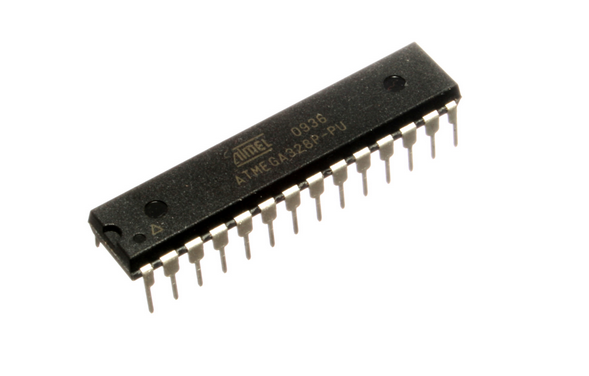
\includegraphics[width = 7 cm]{imagenes/micro.PNG}
    \caption{ATmega 328}
    \cite{atmega}
\end{figure}

\subsubsection{Sensor de obstáculo}
El sensor de obstáculo opera mediante una configuración emisor-receptor de luz infrarroja. Si la luz infrarroja choca contra un obstáculo, esta será reflejada y detectada por el fotodiodo. El rango de detección puede ser configurado mediante los dos controladores. Si no hay un obstáculo en frente la salida del sensor estará en alto, en el momento que se detecte un obstáculo la señal de salida se apagará.

El sensor permite activar o desactivar la detección de obstáculos mediante la manipulación del pin \textit{enable}. Por defecto, el sensor se encuentra en modo activo \cite{obstaculo}.

\begin{figure}[H]
    \centering
    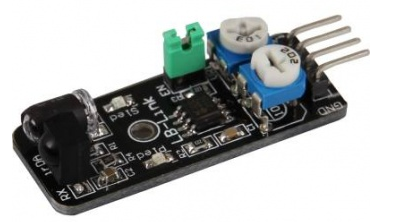
\includegraphics[width = 7 cm]{imagenes/obstacle.PNG}
    \caption{Sensor de obstáculo}
    \cite{obstaculo}
\end{figure}

\subsubsection{Sensor de \textit{traking}}
Es un módulo tipo LEGO, listo para ser conectado al microcontrolador. Se basa en un sensor óptico reflexivo con salida de transistor, el cual se encarga de recibir las señales infrarrojas enviadas para detectar la intensidad de la señal. Con cierto rango de altura, los sensores de pista son ampliamente utilizados para vehículos inteligentes o impresoras para detección de líneas en blanco y negro \cite{track}.

\begin{figure}[H]
    \centering
    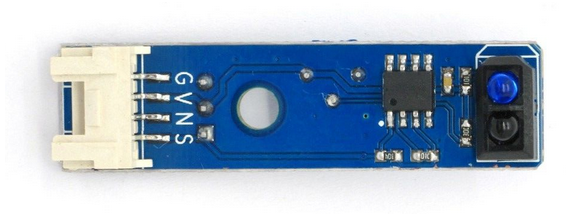
\includegraphics[width = 7 cm]{imagenes/tracking.png}
    \caption{Sensor de pista}
    \cite{track}
\end{figure}


\subsubsection{Motores DC 200 RPM a escala}
Compuesto por un par de motores DC a escala, son usualmente recomendados como una opción barata y sencilla para poner ruedas en movimiento. Requieren una tensión de 4.5V y una corriente sin carga de 190 mA además posee una caja reductora 48:1 y una velocidad de giro de 200 RPM sin carga \cite{motor_dc}.

\begin{figure}[H]
    \centering
    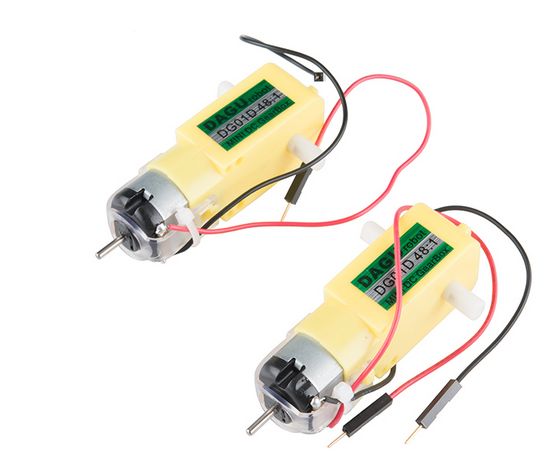
\includegraphics[width = 7 cm]{imagenes/gearmotor.PNG}
    \caption{Hobby Gearmotor - 200 RPM}
    \cite{motor_dc}
\end{figure}

\subsubsection{Módulo de control de motores DC 800 mA}

El módulo de control L9110S 2-Canales es una tarjeta compacta que puede ser utilizada para controlar robots pequeños. Este módulo posee dos controladores independientes capaces de entregar hasta 800 mA en corriente continua. Pueden operar entre 2.5V y 12V lo cual permite que sean usados mediante microcontroladores.

Median de control PWM ---\textit{Pulse Width Modulation}--- es posible controlar la velocidad del motor y una salida digital es usada para indicar la dirección \cite{driver}.

\begin{figure}[H]
    \centering
    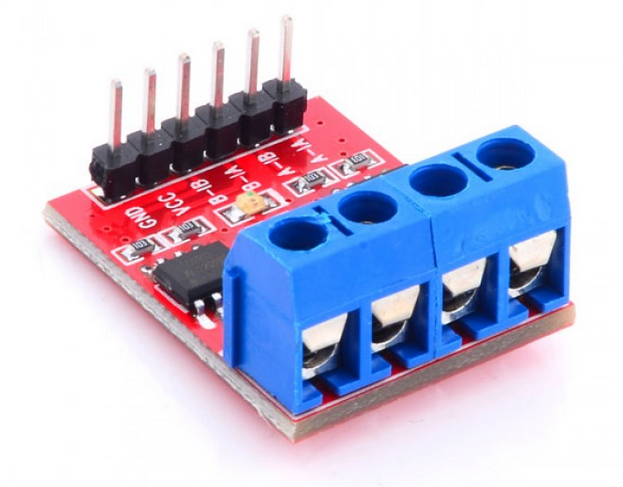
\includegraphics[width = 7 cm]{imagenes/driver.PNG}
    \caption{L9110S Drive Dual Motor DC 800mA}
    \cite{driver}
\end{figure}


\subsubsection{Servomotor}
El servo es un tipo de motor que funciona paso-a-paso, es decir, su giro se determina en ángulos y no en RPM. Pequeño, liviano y con una alta potencia de salida; este tipo de servomotor es capaz de rotar hasta 180 grados \cite{servo}.

\begin{figure}[H]
    \centering
    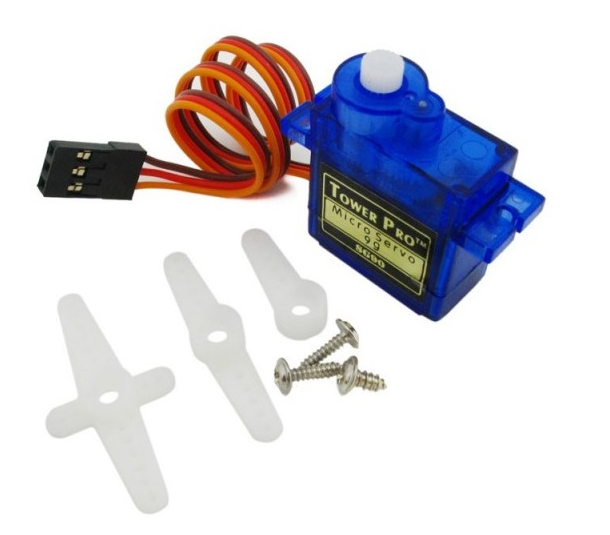
\includegraphics[width = 7 cm]{imagenes/servo.PNG}
    \caption{Servomotor SG90}
    \cite{servo}
\end{figure}

\subsubsection{Piezo Speaker}
Es un pequeño parlante redondo de 12mm el cual opera en todo el rango audible. Pueden ser utilizados para crear interfaces simples musicales. Requiere de una tensión entre los 3.5V y 5V con una corriente media de 35 mA además de una onda cuadrada para su correcto funcionamiento.

\begin{figure}[H]
    \centering
    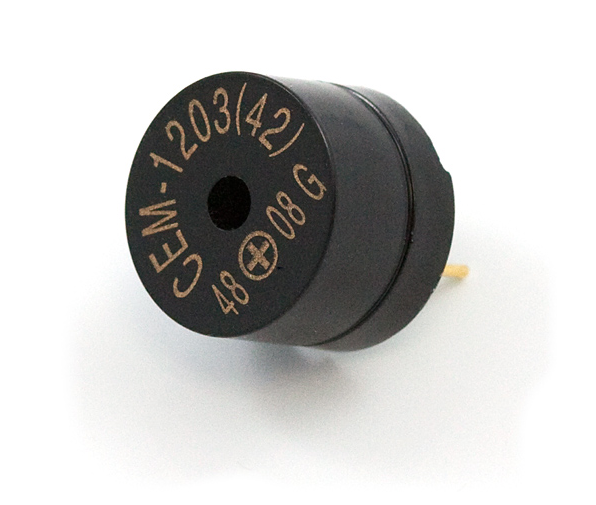
\includegraphics[width = 7 cm]{imagenes/speaker.PNG}
    \caption{Magnetic buzzer}
    \cite{speaker}
\end{figure}


\subsubsection{Módulo bluetooth HC-05}
El módulo bluetooth HC-05 se utiliza en este proyecto para poder enviar datos desde un programa en C al arduino, la comunicación se realiza a través del puerto serial, mediante el cual se transmiten los datos. Dichos datos son interpretados por el arduino para llevar a cabo las funciones que el vehículo realiza. 
\begin{figure}[H]
    \centering
    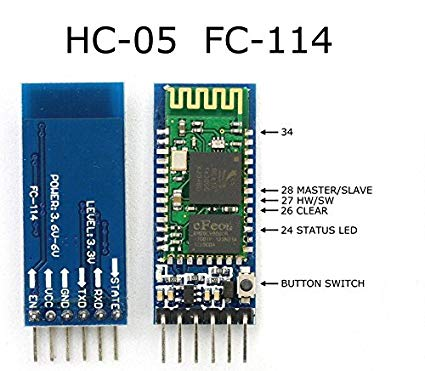
\includegraphics[width= 7 cm]{./imagenes/hc-05.jpg}
    \caption{Módulo bluetooth \cite{bluetooth}}
   
\end{figure}


\subsubsection{Esquemático de conexiones de vehículo}

\begin{figure}[H]
    \centering
    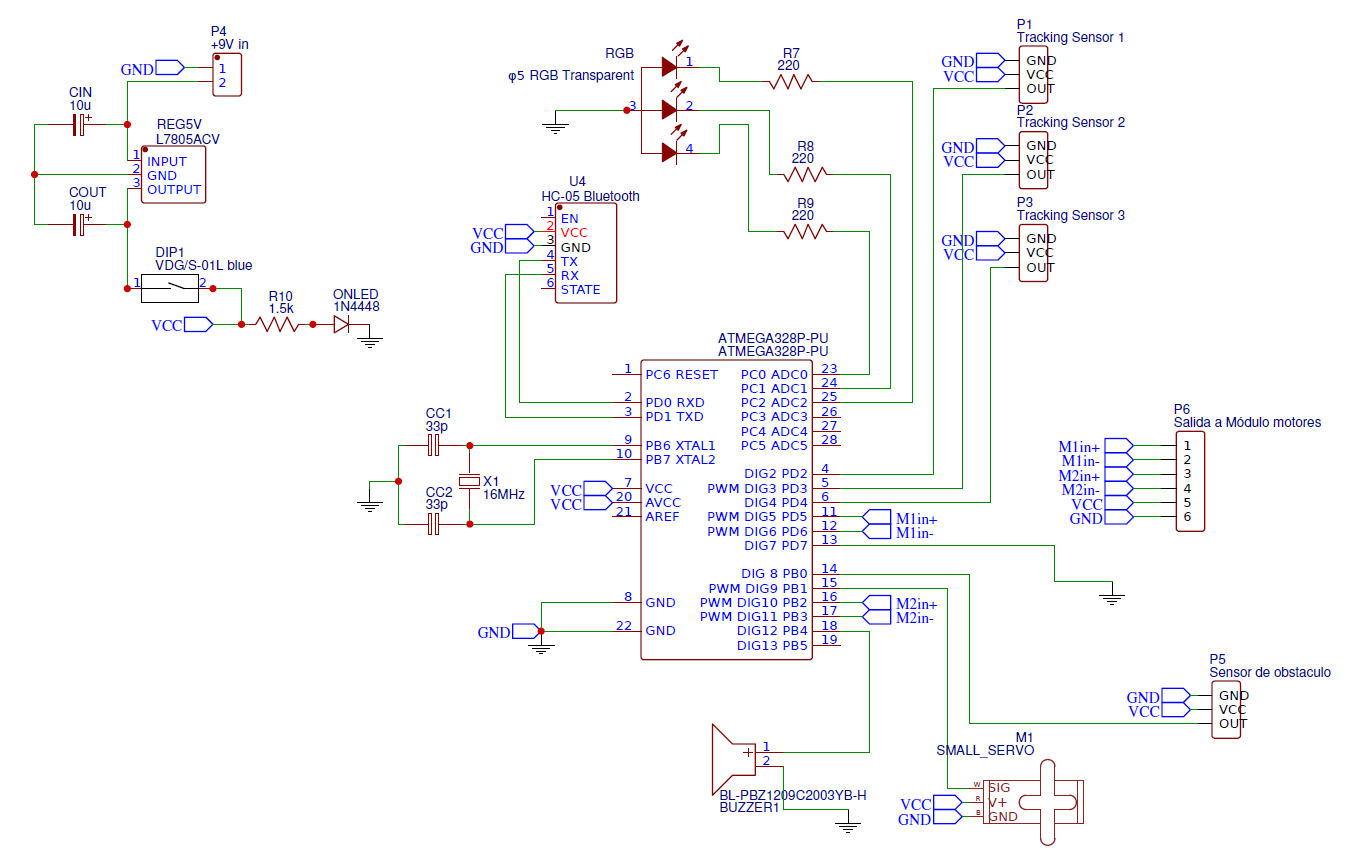
\includegraphics[width = 18 cm]{imagenes/schem_vehiculo.PNG}
    \caption{Esquemático del Vehículo Seguidor de Línea}
\end{figure}



